\documentclass{scrartcl}

% neccesarry for style
\usepackage[english]{babel}
\usepackage[utf8]{inputenc}
\usepackage[T1]{fontenc}
\usepackage{lmodern}

% tools for text
\usepackage{csquotes}
\usepackage{url}
\usepackage{hyperref}

% graphics
\usepackage{graphicx}
\usepackage{xcolor}
\usepackage{tikz}

% maths
\usepackage{amsmath,amssymb,amstext,amsthm}

% programming
\usepackage{listings}

\usepackage{wasysym} %lightning

\input{required/settings.tex}
\input{required/commands.tex}

\renewcommand{\labelenumi}{\alph{enumi})}
\begin{document}
	\begin{center}
		\LARGE
		Information Integration -- Exercise 3 -- Gabriel Glaser
	\end{center}
	\section*{Task 1: Materialized and Virtual Integration}
	\begin{center}
		\fbox{
			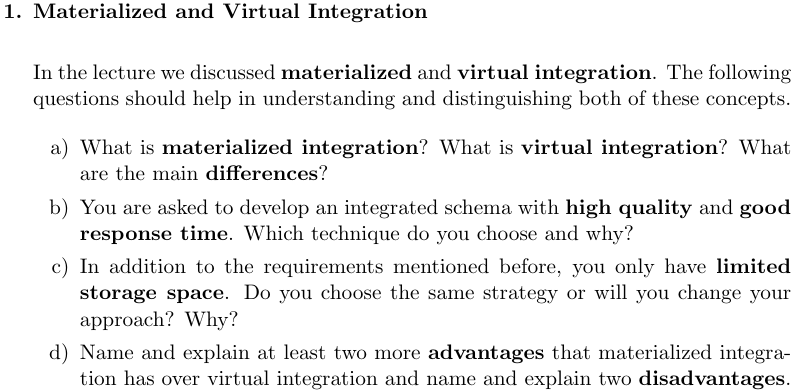
\includegraphics[width=0.9\textwidth]{figures/task1_description.png}
		}
	\end{center}
	\begin{enumerate}
		\item\phantom{phantom}
		\begin{itemize}
			\item
			\textit{Materialized integration} means performing the integration before any user can query the integrated system.
			Therefore, all data (from the sources) has to be extracted at once and is stored using the (global) schema.
			Also, needs further techniques like periodic new data import and various data maintenance processes (e.g., deletion of old data).
			
			\item
			In contrast, \textit{virtual integration} means performing the integration part as soon as a user queries the \enquote{integrated} system.
			Thus, only relevant (with respect to the query) data is retrieved from the sources (using the query language of each source).
			Also, the retrieved data (in source schema) is dropped as soon as the query handling is finished.
			Finally, needs further techniques like handling of source unavailability.
		\end{itemize}
		
		\item
		In this case, materialized integration is a good choice.
		On the one hand, it is capable of producing high quality results, because it is possible to apply many cleaning steps and consider many sources without a user waiting during all computations.
		On the other hand, it can be queried with low response times, because all computations have already been done before the system can be queried.
		
		\item
		This requirement may change the choice, because using materialized integration consists of the step of copying all data of all sources into an own storage.
		If the needed storage is higher than the given storage space limit, virtual integration has to be used instead.
		\newpage
		\item\phantom{phantom}
		\begin{itemize}
			\item An advantage of materialized integration is that (if the building of the system has  finished) it doesn't rely on the availability of the sources anymore.
			Also, it materialized integration is usually more complete, because extracting all data (relevant to a query) for each query is expensive.
			
			\item However, data of materialized integration may not be fresh and changes to the global schema requires transformations on the whole integrated data base.
		\end{itemize}
	\end{enumerate}
	
%	\section*{Task 2: Schema Integration}
%	\begin{center}
%		\fbox{
%			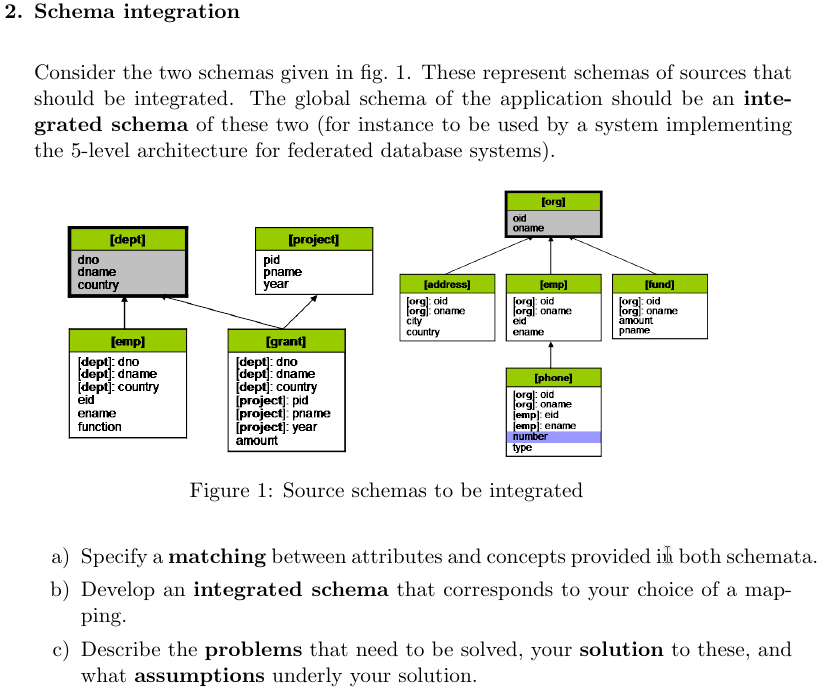
\includegraphics[width=0.9\textwidth]{figures/task2_description.png}
%		}
%	\end{center}
%	\begin{enumerate}
%		\item Found same labels from left source and right source:
%		\begin{center}
%			\begin{tabular}{|r|l|}
%				\hline
%				\textit{Left Source} & \textit{Right Source}\\
%				\hline
%				[dept].country & [address].country\\\relax
%				[project].pname & [fund].pname\\\relax
%				[emp] & [emp]\\\relax
%				[emp].eid & [emp].eid\\\relax
%				[emp].ename & [emp].ename\\\relax
%				[grant].amount & [fund].amount\\
%				\hline
%			\end{tabular}
%		\end{center}
%		\item
%		\item
%	\end{enumerate}
	
	\section*{Task 3: Architectures}
	\begin{center}
		\fbox{
			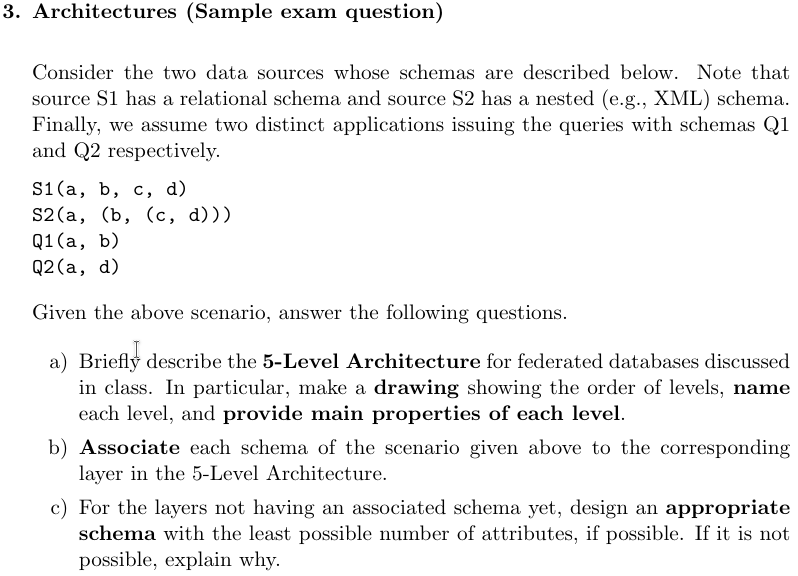
\includegraphics[width=0.9\textwidth]{figures/task3_description.png}
		}
	\end{center}
	\begin{enumerate}
		\item The 5-Level architecture extends the 4-Level architecture by the \textit{component schema} which is a transformation of the \textit{local schema}.
		It is needed to help overcoming heterogeneities.
		The remaining parts of this architecture are...
		\begin{itemize}
			\item \textit{external schemas} of federated schema to be able to offer different schemas to different applications.
			\item \textit{federated schema} which consists of a subset of all attributes of all sources. (in the form of a different schema)
			\item \textit{export schemas} to implement access restrictions or leave out unnecessary data. (for each source)
		\end{itemize}
		\begin{center}
			\hspace*{-1.5cm}
			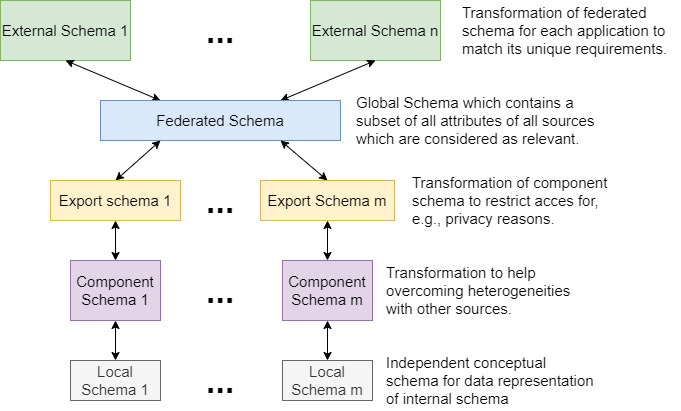
\includegraphics[width=1.1\textwidth]{figures/Task3_a_Visualization.png}
		\end{center}
	
		\item\phantom{phantom}
		\begin{itemize}
			\item \textit{S1} = (a, b, c, d): This scheme likely is a \textbf{component schema}, because it is relational.
			Therefore, heterogeneities can be handled easier when considering the step of federation.
			(However, it could also be a local schema, in case a local source already used a relational schema or even an export schema, if it already contains access restrictions of a relational component schema)
			
			\item \textit{S2} = (a, (b, (c, d))): This scheme likely is a \textbf{local schema}, because hierarchical schemas are (often) difficult to handle during the process of overcoming heterogeneities.
		\end{itemize}
	
		\item Schemas for remaining layers:
		\begin{itemize}
			\item \textit{Local Schema} for \textit{S1}: (a, (b, c), d).
			\item \textit{Component Schema} for \textit{S2}: (a, b, c, d)
			\item \textit{Export Schema} for both \textit{S1}, \textit{S2}: (a, b, d)
			\item \textit{Federated Schema}: (a, b, d)
			\item \textit{External} Schema for \textit{Q1}: (a, b); for \textit{Q2}: (a, d)
		\end{itemize}
		\begin{center}
			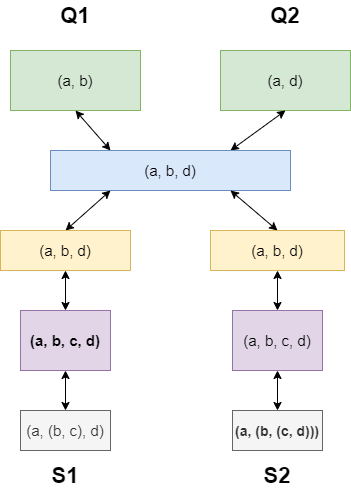
\includegraphics[width=0.7\textwidth]{figures/Task3_c_Visualization.png}
		\end{center}
		No problems.
	\end{enumerate}
	
\end{document}
